%%%%%%%%%%%%%%%%%%%%%%%%%%%%%%%%%%%%%%%%%
% Structured General Purpose Assignment
% LaTeX Template
%
% This template has been downloaded from:
% http://www.latextemplates.com
%
% Original author:
% Ted Pavlic (http://www.tedpavlic.com)
%
% Note:
% The \lipsum[#] commands throughout this template generate dummy text
% to fill the template out. These commands should all be removed when 
% writing assignment content.
%
%%%%%%%%%%%%%%%%%%%%%%%%%%%%%%%%%%%%%%%%%

\documentclass{article}

\usepackage{fancyhdr} % Required for custom headers
\usepackage{lastpage} % Required to determine the last page for the footer
\usepackage{extramarks} % Required for headers and footers
\usepackage{graphicx} % Required to insert images
\usepackage[utf8]{inputenc}

% Margins
\topmargin=-0.45in
\evensidemargin=0in
\oddsidemargin=0in
\textwidth=6.5in
\textheight=9.0in
\headsep=0.25in 

\linespread{1.1} % Line spacing



\setlength\parindent{0pt} % Removes all indentation from paragraphs

%----------------------------------------------------------------------------------------
%	DOCUMENT STRUCTURE COMMANDS
%	Skip this unless you know what you're doing
%----------------------------------------------------------------------------------------

% Header and footer for when a page split occurs within a problem environment
\newcommand{\enterProblemHeader}[1]{
\nobreak\extramarks{#1}{#1 continued on next page\ldots}\nobreak
\nobreak\extramarks{#1 (continued)}{#1 continued on next page\ldots}\nobreak
}

% Header and footer for when a page split occurs between problem environments
\newcommand{\exitProblemHeader}[1]{
\nobreak\extramarks{#1 (continued)}{#1 continued on next page\ldots}\nobreak
\nobreak\extramarks{#1}{}\nobreak
}

\setcounter{secnumdepth}{0} % Removes default section numbers
\newcounter{homeworkProblemCounter} % Creates a counter to keep track of the number of problems

%----------------------------------------------------------------------------------------
%	NAME AND CLASS SECTION
%----------------------------------------------------------------------------------------

\newcommand{\lessonNumber}[1]{Lezione\ \##1} % Assignment title
\newcommand{\lessonDate}[4]{#1,\ #2\ #3\ #4} % Due date
\newcommand{\lessonCourse}[1]{#1} % Course/class
\newcommand{\lessonTime}[1]{#1} % Class/lecture time
\newcommand{\lessonTeacher}[1]{#1} % Teacher/lecturer
\newcommand{\lessonAuthor}[1]{#1} % Your name
\begin{document}

\section{Diagrammi di sequenza (5)}

Descrivono la collaborazione di un gruppo di oggetti che devono implementare collettivamente un comportamento.

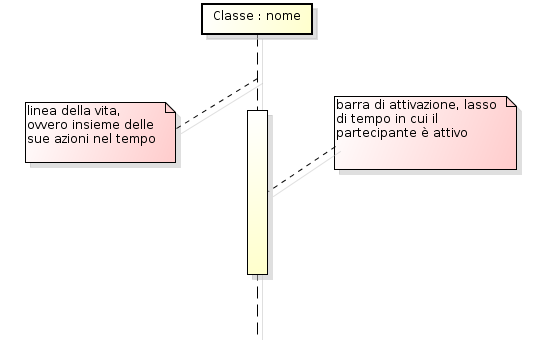
\includegraphics[width=0.5\columnwidth]{img6} % Example image


Le iterazioni tra più partecipanti avvengono tramite \textbf{messaggi}. L'inizio di un messaggio si rappresenta con una freccia continua da un partecipante all'altro. E' possibile avere anche un messaggio che arriva dall'\textbf{esterno} del partecipante. L'evento esterno attiva il diagramma di sequenza e lo fa partire. Il ritorno di un messaggio è rappresentato da una freccia tratteggiata.\\
Esistono due possibili messaggi: 
\begin{itemize}
	\item \textbf{Asincroni}
	\item \textbf{Sincroni}
\end{itemize}

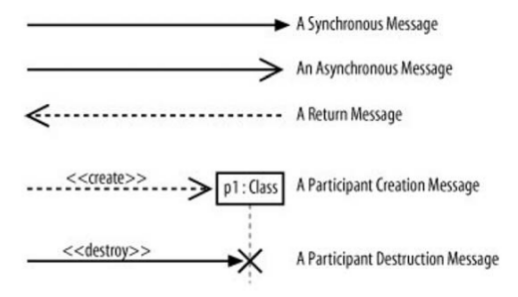
\includegraphics[width=0.5\columnwidth]{img5} % Example image


Un partecipante può creare un altro partecipante (normalmente tramite la \textit{new}), per questo si usa la \textbf{create}:

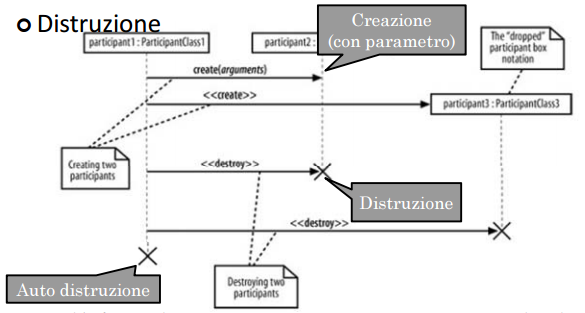
\includegraphics[width=0.5\columnwidth]{img7} % Example image


Di contro un oggetto può richiedere la distruzione di un altro oggetto. In questo caso si invia un altro messaggio e si mette una X sulla linea della vita del partecipante. Un oggetto può anche autodistruggersi.\\

Se ho bisogno di modellare la collaborazione uso i diagrammi di sequenza, se devo modellare algoritmi uso i diagrammi di attività.\\
Controllo \textbf{centralizzato} e \textbf{distribuito}. Bisogna cercare di delegare il più possibile agli oggetti le operazioni su se stessi (\textit{delegation pattern}. Nel contratto distribuito non abbiamo più un registro che \textit{schedula} tutte le attività, ma tutto parte da un singolo oggetto che invoca metodi su altri oggetti, manda e riceve messaggi.\\


\end{document}